\chapter{Membuat Aplikasi Akademik dengan APEX Oracle Online}

\section{Membuat Workspace}
Sebelum membuat aplikasi akademik menggunakan APEX Oracle online, buatlah terlebih dahulu workspace yang akan digunakan untuk membuat aplikasi tersebut. Berikut ini adalah cara membuat workspace APEX Oracle.
\begin{enumerate}
    \item Buka website APEX Oracle online .
    \item Login akun oracle anda
    \item Setelah login kita akan menuju ke halaman Request a Workspace.

\begin{figure}[!htbp]
    \centering
    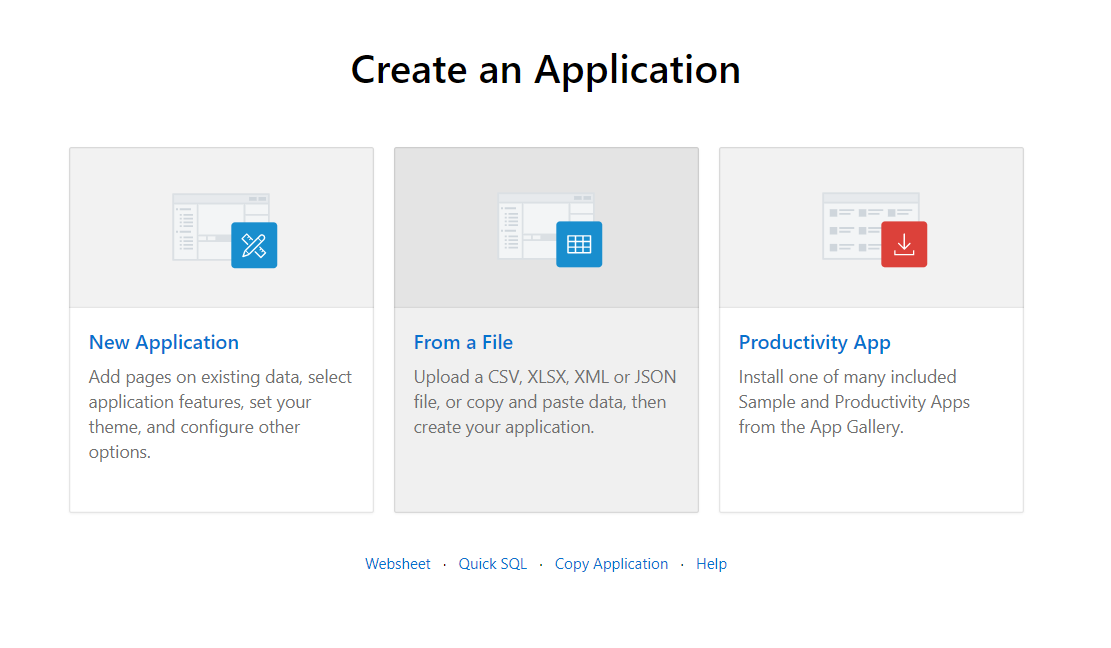
\includegraphics[scale=0.5]{gambar/1.png}
    \label{penanda}
\end{figure}

    \item Untuk mengisi identification, masukan first name, last name, email, dan nama workspace yang akan dibuat.
    \item Pada survey, klik yes pada kedua pertanyaan seperti gambar berikut ini.
    \item Setelah survey, isi justification dan klik next
    \item Lalu, pada agreement klik i accept the terms dan klik next.
    \item Selanjutnya confirmation dan submit workspace yang akan dibuat.

\end{enumerate}

\section{Konfirmasi Email Workspace}
Simak dibawah ini cara mengonfirmasi email untuk membuat workspace.
\begin{enumerate}
    \item Buka email dan klik kotak masuk
    \item Klik email dari apex oracle
    \item Berikut ini adalah tampilan email dari apex oracle.
    \item Setelah workspace berhasil dibuat, masukkan password untuk workspace yang telah dibuat tadi
    \item Workspace berhasil dibuat
\end{enumerate}

\section{Membuat Aplikasi Akademik dari Data Excel}
Berikut ini adalah cara membuat aplikasi akademik dari data excel.

\begin{enumerate}
    \item Setelah sig in ke workspace APEX Oracle, klik app builder
    \item Pada halaman app builder, klik create untuk membuat aplikasi
    \item Arahkan kursor ke from a file untuk mengupload data excel
    \item Selanjutnya drop file excel
    \item Setelah file di drop, input nama table, dan load data
    \item Setelah table dibuat, klik create application
    \item Input nama aplikasi, aplikasi ini saya namakan aplikasi akademik.
    \item Lalu, klik check all dan create application
    \item Setelah aplikasi terbuat, running aplikasi dengan klik run application
    \item Aplikasi akan berjalan dan mengarah ke halaman baru. Untuk membuka aplikasi, log in terlebih dahulu menggunakan user APEX Oracle dan password pada workspace yang digunakan.
    \item link : https://apex.oracle.com/pls/apex/f?p=79096:LOGIN\_DESKTOP:102401395122138:::::
\begin{figure}[!htbp]
    \centering
    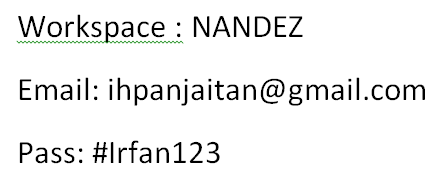
\includegraphics[scale=1]{gambar/2.png}
    \label{penanda}
\end{figure}
\end{enumerate}